\chapter{Analysis strategy and event selection} %day1
\label{chap:selection}

Given the theoretical motivation for \BSM physics in
Chapter~\ref{chap:theory}, the next Chapters of this thesis describe a
search for \SUSY with the \CMS detector in $13~\tev$ proton collisions
produced by the \LHC. The analysis is designed to target \SUSY
produced in a strong force interaction that decays hadronically via
\SM particles to a weakly interacting \LSP. The typical \SUSY models
considered in this search are those with gluino or squark pair
production. However, it is possible to generalise the search to look
for any \BSM signatures that have a weakly interacting particle with
significant momentum in the final state.
% introduce analysis and what the next chapters are about
% hadronic, inclusive, targets gluino and squark production but can be
% generalised to DM

As \SUSY has a significant number of free parameters, it can manifest
itself in a wide range of decay topologies. For this reason the
analysis is aimed to be as inclusive as possible, covering as much
parameter space as is feasible.  This is dictated by an ability to
predict the backgrounds from \SM processes with minimal uncertainties.
The search then attempts to find statistically significant excesses in
the data counts above those predicted for the various backgrounds. To
maximise the chance of seeing \BSM phenomena events are typically
required to have significant hadronic activity and missing momentum.  
% Robust strategy - minimise background uncertainties and look for
% excesses on top, in a conservative way (be very general here)


%%%%%%%%%%%%%%%%%%%%
\section{Challenges for a hadronic \BSM search}
\label{sec:challenge}

%main challenge in limiting and understanding backgrounds
The main challenge for a hadronic \BSM search is in limiting and
understanding the backgrounds, while maximising acceptance of a wide
range of potential \BSM signals. Within the analysis presented in this
Chapter the backgrounds are considered in two separate categories,
either as coming from a QCD multijet process or from a \SM process
with genuine \MET. As the search can look for generic signs of
excesses that are indicative of \BSM processes, considerations of the
modelling of the signal models are not as important as constraining
and understanding these backgrounds.

\subsection{The QCD multijet background}
\label{sec:qcdMultijet}

The most abundant \SM process in $pp$-collisions at the \LHC is \QCD
multijet production through strong force interactions. This background
is orders of magnitude greater than other processes, as is evident
from the total \LHC cross section in Fig.~\ref{fig:xsecs}. The
majority of the \QCD background consists of events with multiple jets,
most commonly two, produced in a balanced configuration, with no
significant missing momentum, \MET or \MHT. A requirement on these
variables therefore significantly reduces the background. As
the abundance of such events is so large, however, mismeasurement of
the jets can lead to a significant \QCD background passing such
requirements. The fake missing energy can be introduced in a variety
of ways:
\begin{itemize}
\item{Effects in the detector leading to inefficiencies, such as jets
falling into regions of the detector that or uninstrumented or have a
reduced response due to hardware issues.}
\item{Fake additional energy being introduced. This can occur through
detector malfunctions, for example from problems in the readout
electronics. It can also be introduced through \PU that is attributed to
the primary vertex. Additionally beam interactions that produce
particles outside the detector can lead to mismeasurement.}
\item{Issues at the reconstruction stage can also introduce fake \MET,
such as through under or over-corrections of jet energies, or through
the reconstruction algorithms missing physics objects that are
produced.}
\item{Physics objects with energies that fall below their selection
threshold can also artificially introduce missing energy signatures,
particularly when there is a collection of them pointing in a similar
direction.}
\end{itemize}

The ways in which this fake missing energy can be introduced are
taken account of in as many ways as possible. However, due to the
nature of these effects, which is often time dependent, they cannot be
fully accounted for in simulation. This fact, coupled with the
difficulty in accurately simulating \QCD processes due to theoretical
uncertainties, makes constraining the multijet background a significant
challenge. 

It is also possible for the \QCD multijet background to be produced in
association with genuine \MET. This occurs in the case of \emph{heavy
flavour} \QCD, where a $b\bar{b}$ quark pair are produced and at least
one the $b$-quarks decay via the weak force, producing a neutrino.
This is subdominant to the mismeasured multijet background, but must
still be accounted for. 
% heavy flavour qcd

% relevant to the trigger (cite back advantages from trigger chapter)

\subsection{Backgrounds from standard model processes with genuine
\MET}

The other class of \SM backgrounds are those produced with genuine
\MET. These processes only occur in the \SM through the electroweak
production of neutrinos and can be denoted as \emph{EWK}. Due to the
mass scale of such electroweak processes, they commonly occur in
association with jets of a significant momentum. The dominant
processes that constitute this background are \wj, \znunu and \ttbar,
with residual backgrounds from other, lower cross section,
vector-boson or top production processes.

As a hadronic analysis does not look for leptons in the final state,
vetoing isolated leptons can help to reduce the background from the
\wj and \ttbar processes. In these cases a lepton is always produced
in association with the neutrino that results in the significant \MET.
Such events will only present a problem when the leptons are not
reconstructed, or do not appear to be isolated.  If the $W$ boson
decays via a \tau-lepton that subsequently decays hadronically the
event will not be removed by the lepton veto.  This is a comparably
small background, however.

The major irreducible background in \BSM searches with \MET comes from 
\znunu processes. They produce a pure missing energy signature with no
associated leptons to veto. Understanding this background to a high
degree of accuracy constitutes a significant challenge. Due to the
better simulation of electroweak processes compared to \QCD processes,
this background can be understood with smaller uncertainties than the
\QCD background.
% Z nu nu
%plots with backgrounds: http://www.hep.ph.ic.ac.uk/~mc3909/procs/

%%%%%%%%%%%%%%%%%%%%
\section{The \alphat analysis} 

The search for \SUSY described within this thesis revolves around
suppression of the \QCD multijet background to negligible levels
through the use of topological variables, including \alphat,
described in Sec.~\ref{sec:topoVars}. With negligible \QCD the
large uncertainties that are usually prevalent when predicting this
background are greatly reduce. The use of these topological variables
also provides robustness against a wide range of mismeasurement
effects, which are particularly relevant when looking at early data
when the detector is not as well understood. The remaining background
from electroweak processes is then estimated in a \emph{data-driven} way,
minimising the uncertainties from relying on simulation.

During Run~1 of the \LHC the \alphat analysis has been performed
extensively to search for \SUSY. Datasets of $4.98~\ifb$ at
$\sqrt{s}=7~\tev$ and $18.5~\ifb$ at $\sqrt{s}=7~\tev$ have been
analysed, setting limits on \SUSY production within the context of
simplified models
\cite{Chatrchyan:2011zy,Khachatryan:2011tk,Chatrchyan:2012wa,Chatrchyan:2013mys,Khachatryan:2016pxa}.
The analysis presented within this thesis is performed on the data
collected during Run~2 of the \LHC at $\sqrt{s}=13~\tev$. The analysis
has been redesigned and optimised to perform well at the higher centre
of mass energy. Significant improvements have been made to improve the
sensitivity of the analysis and in characterising the various
backgrounds.

%%%%%%%%%%%%%%%%%%%%
\section{QCD multijet suppression with topological variables} %day2
\label{sec:topoVars}

As discussed in Sec.~\ref{sec:qcdMultijet}, a pure requirement on the
\MET of an event is not always enough to remove the \QCD multijet
background.  To effectively remove it, the mismeasurement that leads
to the fake \MET signature must be identified and used to remove
mismeasured events. This can be achieved by making use of topological
variables, which use specific facts about the topology of an event to
decide whether the \MET comes from mismeasurement or a weakly
interacting particle. 
%why topological variables work!! - fake met from detector cock ups

\subsection{The \alphat variable}
%introduce the variables and why they're useful

The dimensionless variable, \alphat, was originally proposed as the
$\alpha$ variable \cite{Randall:2008rw}, but changed to a transverse
quantity to make it more suitable for use in a hadron collider
\cite{CMS-PAS-SUS-08-005,CMS-PAS-SUS-09-001}. It is intrinsically
robust against jet energy mismeasurements in multijet systems. For a
dijet system, \alphat is defined as: 
\begin{equation}
\alpha_T=\frac{E_T^{j_2}}{M_T}, 
\end{equation} 
where $E_T^{j_2}$ is the transverse energy of the lower energy jet and
$M_T$ is the invariant mass of the dijet
system, defined as:
\begin{equation}
M_T=\sqrt{(\Sigma E_T^{j_i})^2-(\Sigma p_x^{j_i})^2-(\Sigma
p_y^{j_i})^2},
\end{equation}
where $E_T^{j_i}$ is the transverse energy of jet, $j_i$ and the $x$
and $y$ components of the transverse momentum are $p_x^{j_i}$ and
$p_y^{j_i}$ respectively.

In the case that the event in question is a perfectly measured dijet
event $E_T^{j_1}=E_T^{j_2}$ and both jets are back-to-back in $\phi$.
This results in a value of $\alphat=0.5$ when the momentum of each jet
is large in comparison with its mass, as is usually the case in
\QCD multijet events. If the jets are still back-to-back but one of
them is mismeasured, this will result in a value of $\alphat<0.5$.
However, in the case that the two jets are recoiling from a genuine
source of \MET, they will not be back-to-back and generally $\alphat>0.5$.

For events with more than two jets, a \emph{pseudo dijet} system is
formed by summing jets vectorially to combine them.  The system chosen
is one that minimises $|\Delta E_T|$, the difference between the $E_T$
of each pseudo jet, where $E_T$ is the scalar sum of the transverse
energies of all the jets in each pseudo jet. This form of clustering
is chosen as it forms the most balanced configuration, making the
pseudo dijet event appear as close to an event with no mismeasurement
as possible. It leads to a generalised form of $\alpha_T$: 
\begin{equation}
\alpha_T=\frac{\Sigma E_T^{j_i}-\Delta
E_T}{2\sqrt{(\Sigma E_T^{j_i})^2-\cancel{H}_T^2}}.
\end{equation} 
In the case that there is no mismeasurement or \MET, $\Delta
E_T=\MET=0$ and $\alphat=0.5$. However, if the energy of the jets is
mismeasured, the value of $\Delta E_T$ will be very close to \MET,
resulting in $\alphat<0.5$. When the jets are recoiling from genuine
\MET, $\Delta E_T\sim 0$ and $\alphat>0.5$.
  
The efficacy of an $\alphat$ cut in removing the \QCD multijet
background is evident in Fig.~\ref{fig:alphaT}. By
choosing an appropriate cut above $0.5$ it is possible to reduce the
multijet background to a negligible level.

\begin{figure}
	\begin{center}
		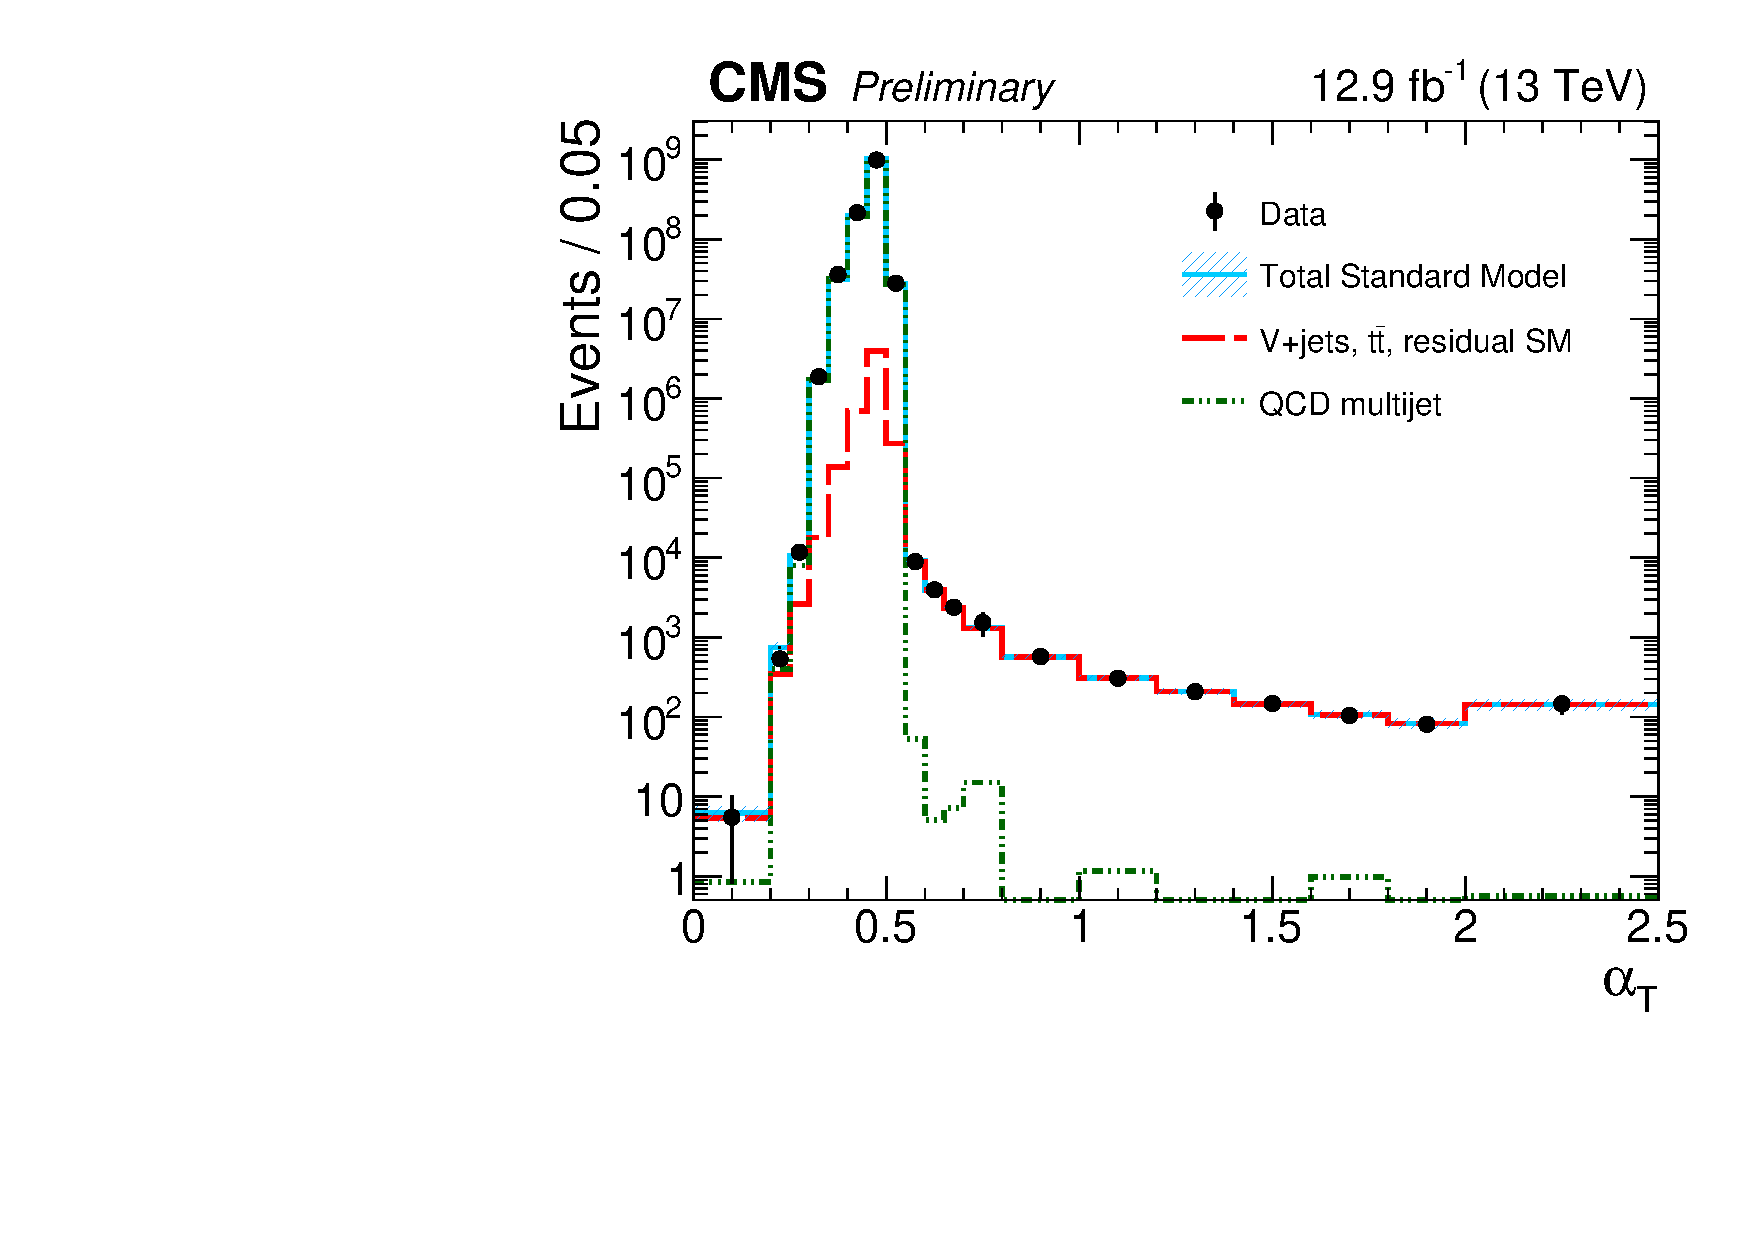
\includegraphics[width=0.7\linewidth]{figs/analysis/eventSelection/CMS-PAS-SUS-16-016_Figure-aux_001}%alphaT1_bkgd}
	\end{center}
  \caption{The $\alpha_T$ distribution for events with $H_T>200$ GeV
  that pass the pre-selection criteria (Sec.~\ref{sec:preselection}) when
  $\alphat<0.55$ and the signal selection criteria
  (Sec.~\ref{sec:signalregion}) when
  $\alphat>0.55$. The green dotted line shows the expected multijet
  QCD background that can be removed with an appropriate cut on
  $\alpha_T$}
	\label{fig:alphaT}
\end{figure}

\subsection{The \bdphi variable}

To further suppress the \QCD multijet background after applying an
\alphat cut the biased-$\Delta\phi$, \bdphi, variable is introduced.
This is a variation on the $\Delta\phi$ variable, which is usually
defined as the minimum azimuthal angle between the \MET and any jet in
the event. When calculating \bdphi, each jet is compared to the
\MHT, but the \MHT is recalculated as if the jet were not present in
the event. This leads to the definition:
\begin{equation}
\bdphi = \rm{min}(\Delta\phi(\vec{p_T^{j_i}},\vec{\MHT^{j_i}})),
\end{equation}
where $vec{\MHT^{j_i}}=\vec{\MHT}+\vec{p_T^{j_i}}$. The removal of the
probe jet from the event adds robustness to over-measurement, as well
as under-measurement, of the jet energies.
% introduce and explain

The \bdphi variable acts to remove events in which the \MET is
collinear with the jets, a typical feature of mismeasurement. However,
it also helps to remove the heavy flavour \QCD multijet background,
where a $b\bar{b}$ pair is produced and decays leptonically, producing
neutrinos. These neutrinos are a genuine source of \MET that are
typically boosted along the jet direction. In these cases the \bdphi
helps to reject the \QCD background that may have passed an $\alphat$
cut. The \bdphi distribution for multijet events and the remaining \SM
backgrounds is shown in Fig.~\ref{bdphi}. A requirement on \bdphi
close to 0.5 will significantly reduce any \QCD background.
%bDPhi augments alphaT when considering mismeasurement in heavy
%flavour qcd stuff
% show the plot from Mark

\begin{figure}
	\begin{center}
		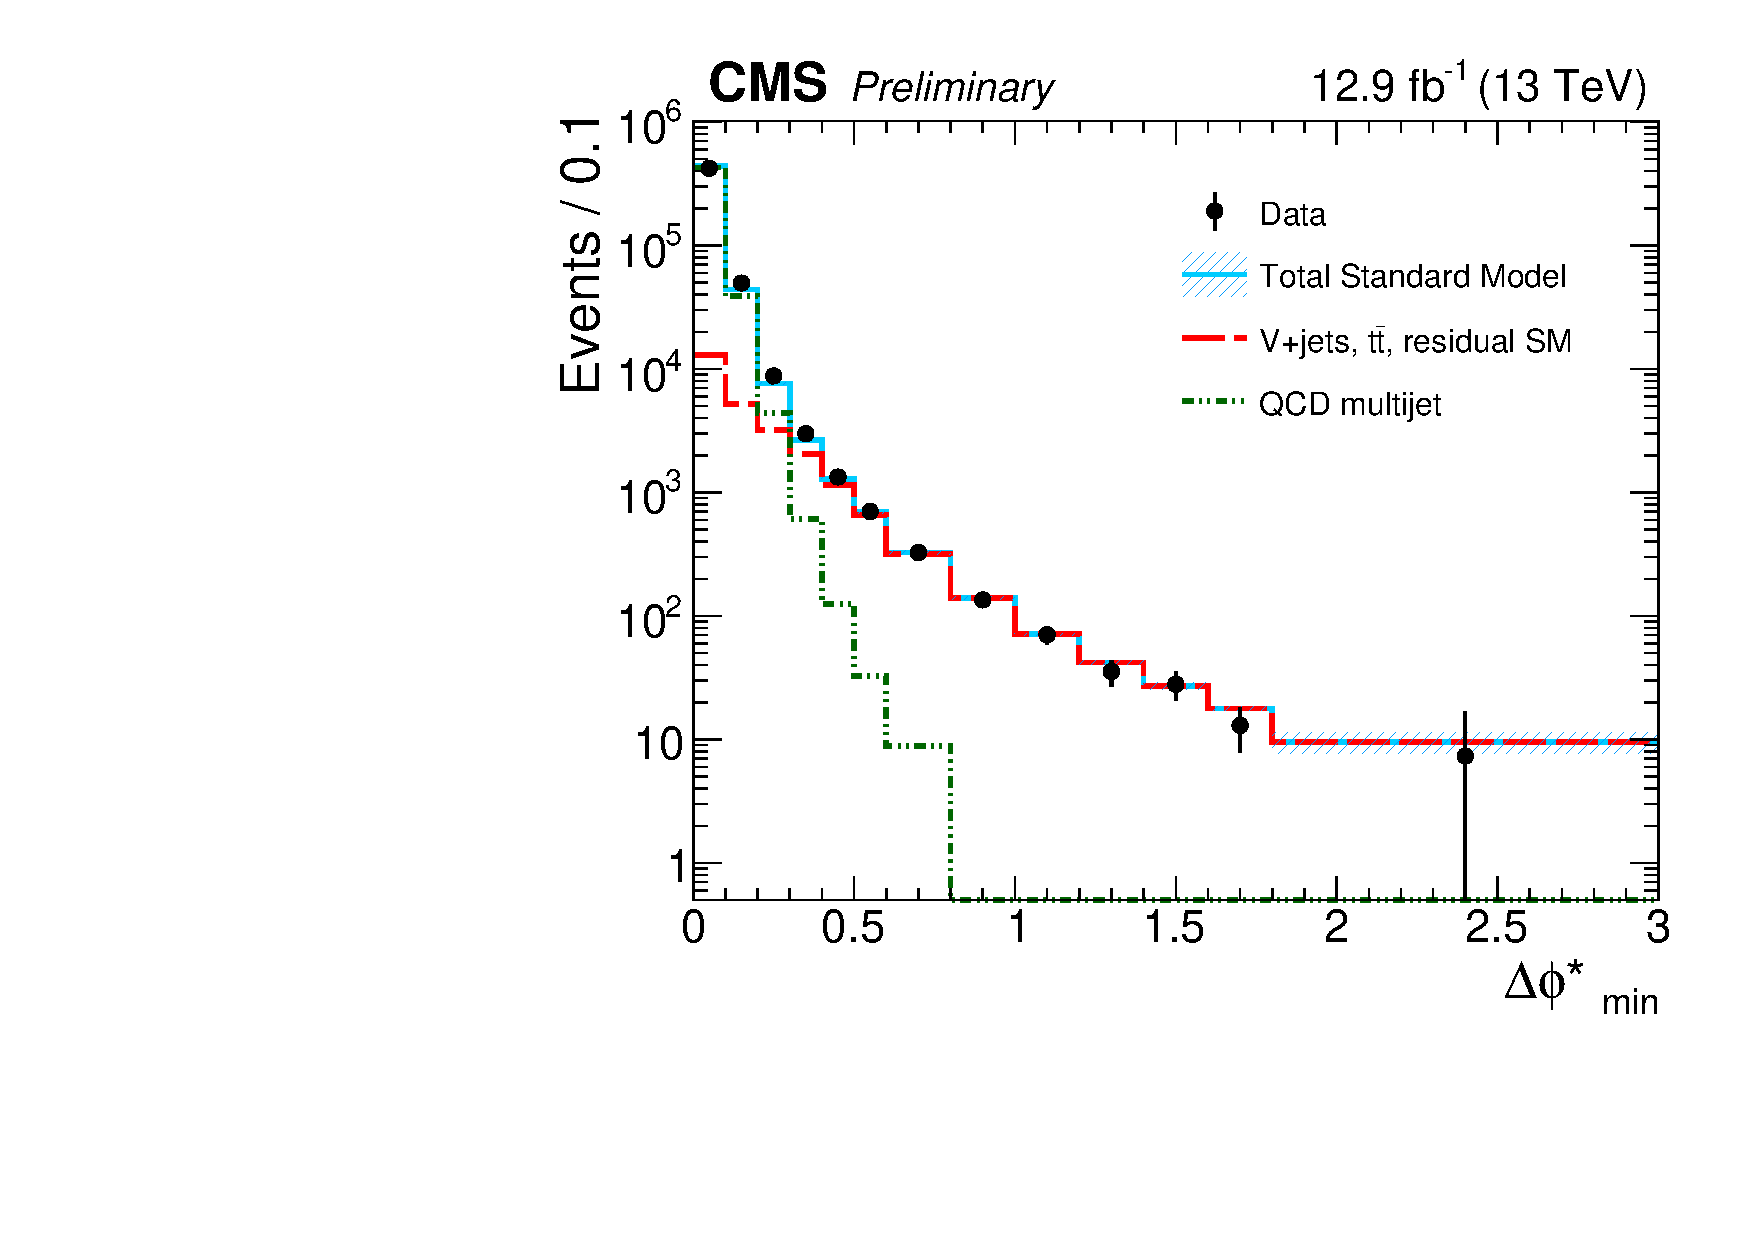
\includegraphics[width=0.7\linewidth]{figs/analysis/eventSelection/CMS-PAS-SUS-16-016_Figure-aux_002}%alphaT1_bkgd}
	\end{center}
  \caption{The \bdphi distribution for events with $H_T>800$ GeV that
  pass the pre-selection criteria (Sec.~\ref{sec:preselection}). The
  green dotted line shows the expected multijet QCD background that
  can be removed with an appropriate cut on $\alpha_T$}
	\label{fig:bdphi}
\end{figure}

%put the stuff about bDPhi over dPhi as in the ICHEP note

In Fig.~\ref{fig:bDPhi_nominal} a comparison of the abilities of the
\bdphi variable to control the \QCD multijet background with a similar
jet-\mht angular variable \dphimhtj, the minimum azimuthal separation
between the \mht-vector and the leading four jets, is presented. The
\bdphi variable exhibits a distribution that is more sharply peaked
for the \QCD multijet background at low values and faster falling than
\dphimhtj,  \dphimhtj for QCD conversely has a broader distribution
with a larger leakage for a comparable azimuthal selection. This
demonstrates the ability of \bdphi to provide a better control of the
\QCD background while retaining acceptance of events with genuine \mht,
in this case represented by the V+jets, \ttbar and other residual SM
backgrounds with genuine \met. 

\begin{figure}[!h]
 \centering
 \subfloat[\bdphi distribution.\label{fig:bDPhi_dist}]{
 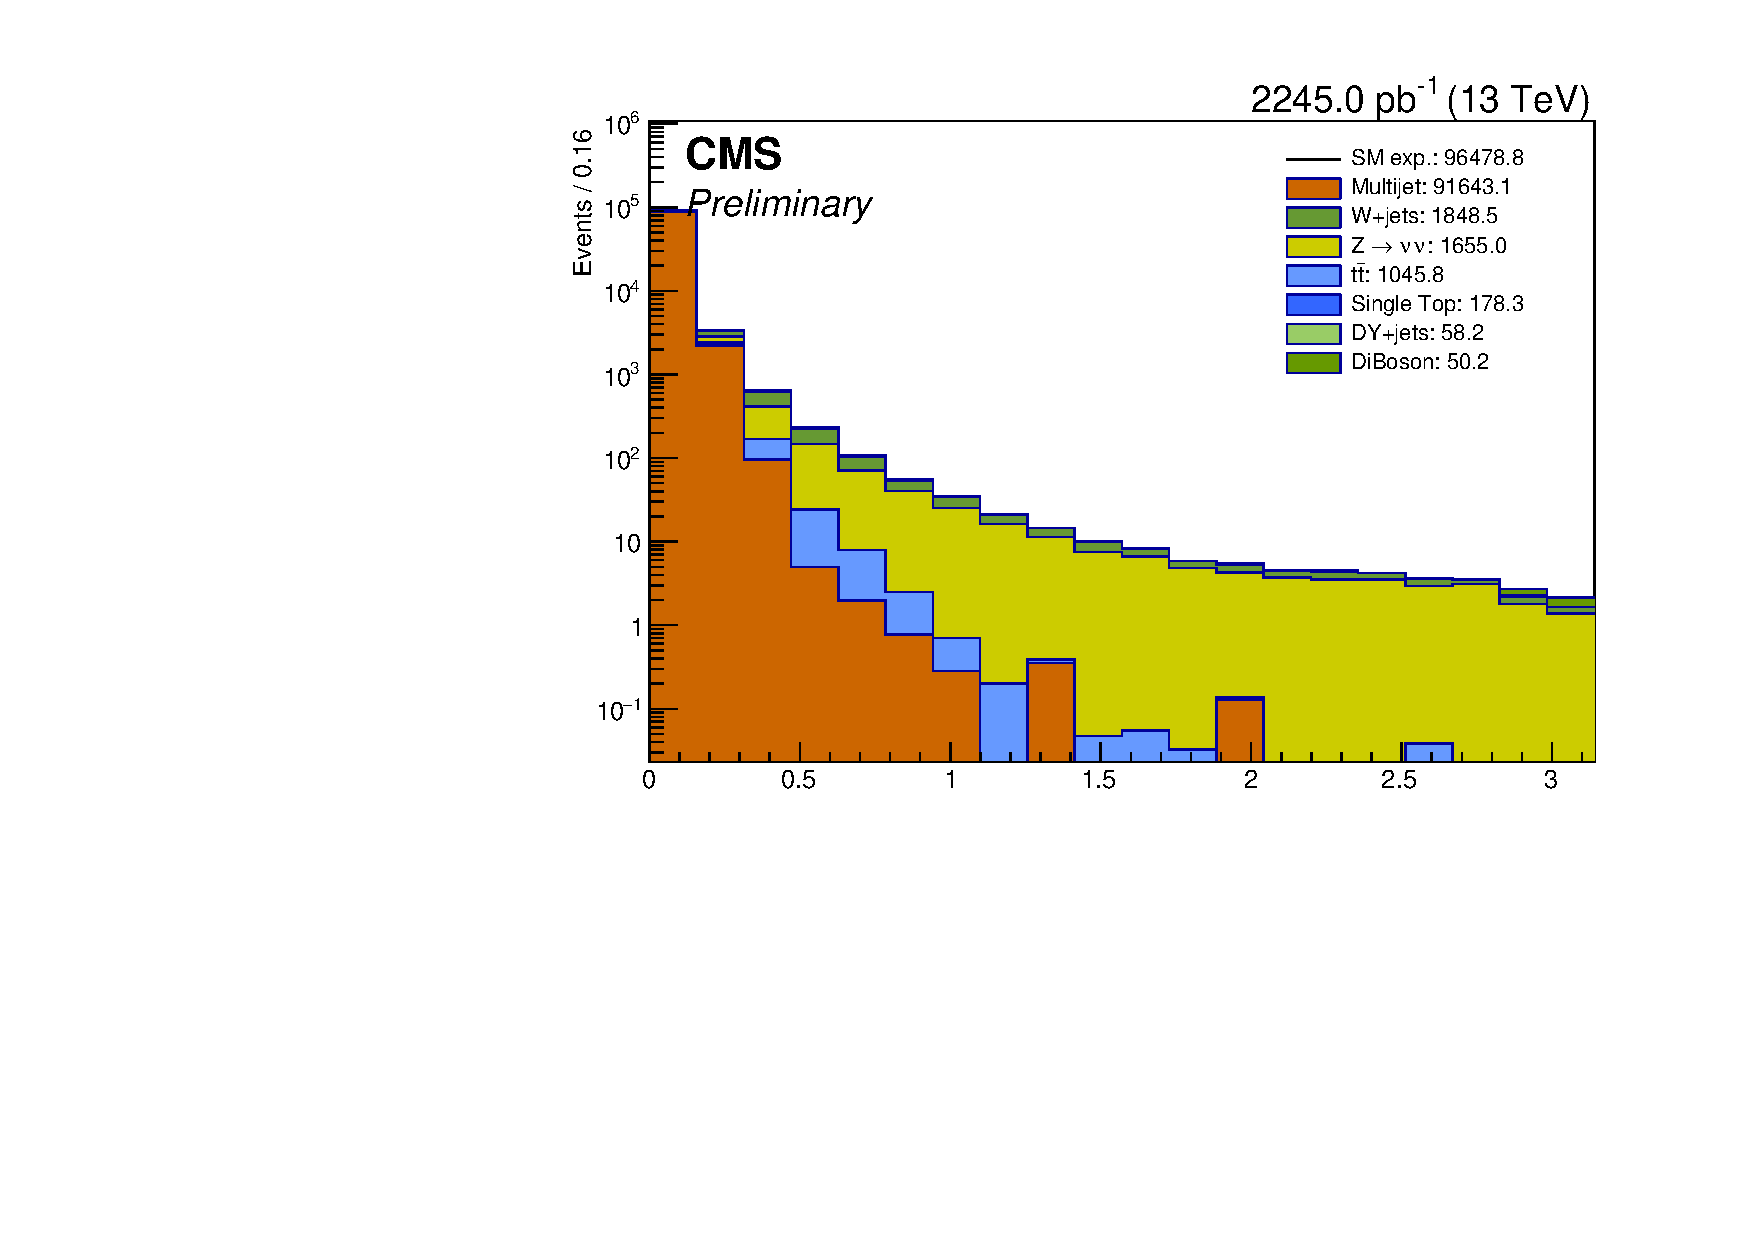
\includegraphics[width=0.5\textwidth]{figs/analysis/eventSelection/biasedDPhi_all_800}
 }
 \subfloat[\dphimhtj distribution.\label{fig:DPhiMht_dist}]{
 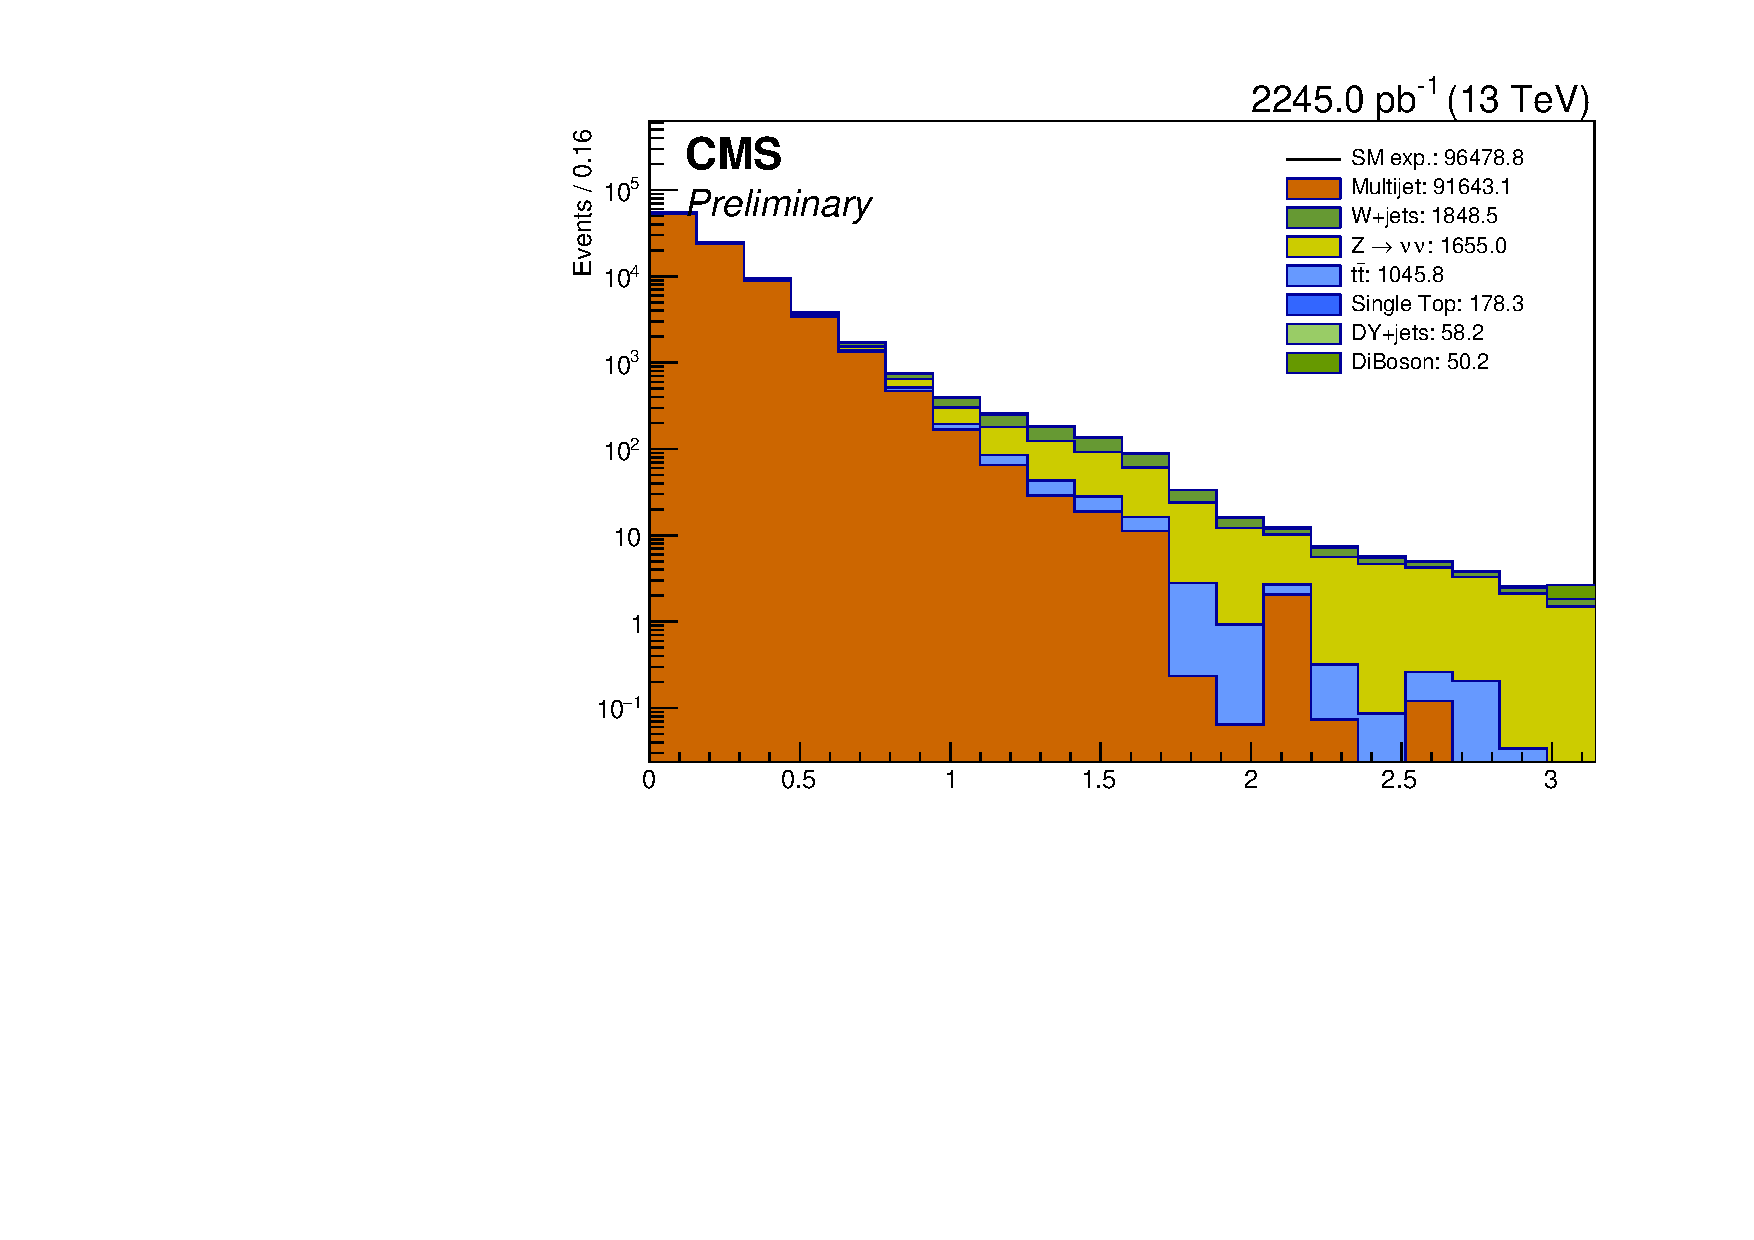
\includegraphics[width=0.5\textwidth]{figs/analysis/eventSelection/minDeltaPhiMht_all_800}
 } \\
 \caption{\bdphi and \dphimhtj distributions of MC simulation of the
 dominant analysis backgrounds
 after analysis selections for \scalht $> 800$ \GeV. }
 \label{fig:bDPhi_nominal}
\end{figure}

This is further demonstrated in Fig.~\ref{fig:bDPhi_roc}, where the
efficiency of retaining processes with genuine \mht is plotted against
the background efficiency for a series of \bdphi, \dphimhtj and
\dphimhtjall cuts, where \dphimhtjall considers all jets rather than
just the leading four. The points with a cut of $0.5$ are highlighted
as stars on the plot. As the general analysis strategy involves reducing
the \QCD multijet background to a negligible level while maximising
signal acceptance, these plots demonstrate that this is most
achievable with a cut on \bdphi. For the same threshold requirement of
$0.5$ on each variable, the \bdphi variable provides an efficiency for
multijet events that is approximately three orders of magnitude lower
than for \dphimhtj at the cost of approximately a factor $3$ reduction
in signal efficiency. The threshold on \bdphi required to give an
approximately equivalent suppression of QCD achieved with the
\dphimhtj variable is larger than 1.5, at the cost of a loss of a
factor $5$ in signal acceptance w.r.t. \bdphi. This also holds true in
the extreme case of a high jet multiplicity signal model.
Additionally, despite performing similarly to \bdphi for separating
the non-multijet from multijet backgrounds, the \dphimhtjall variable
performs worse for a high jet multiplicity signal model than \bdphi.

\begin{figure}[!h]
 \centering
 \subfloat[Acceptance of SM backgrounds with genuine \met vs QCD
 acceptance]{
 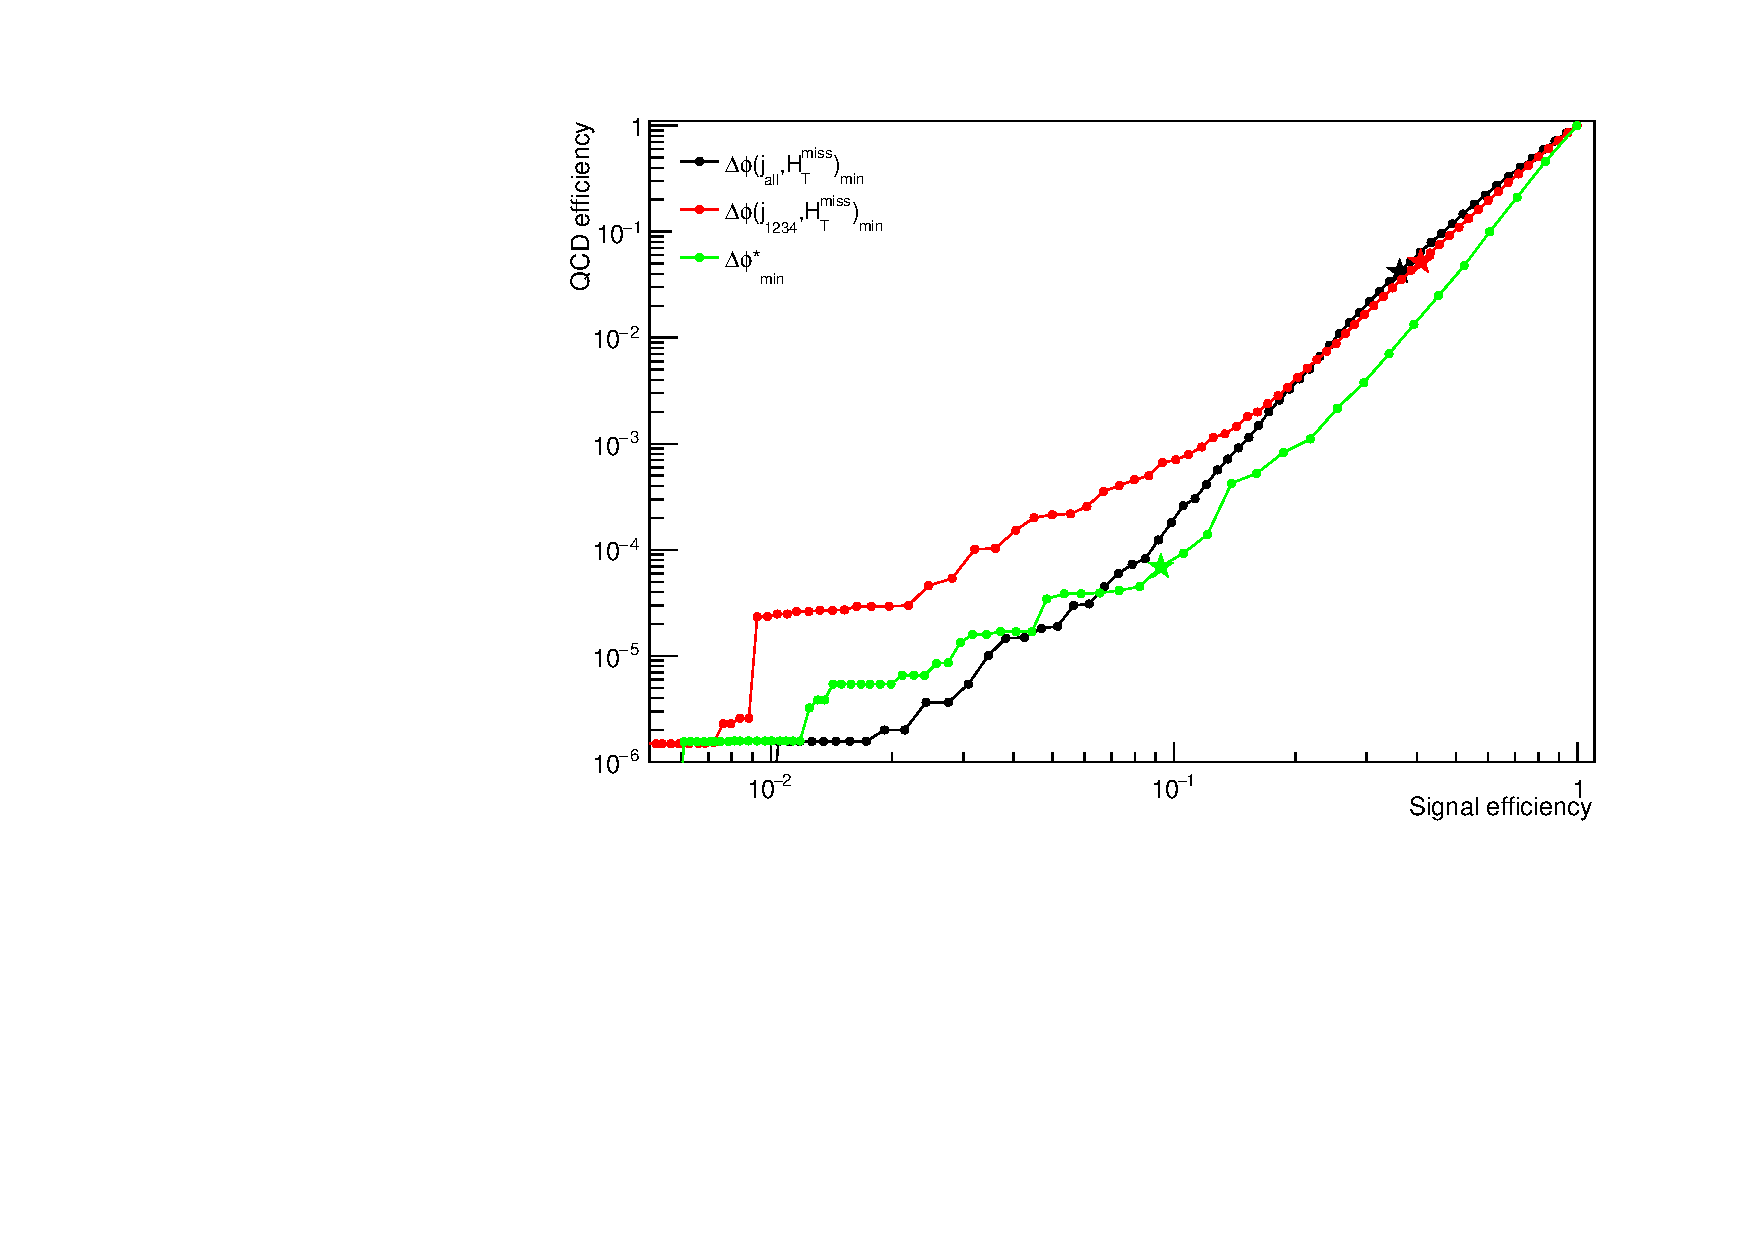
\includegraphics[width=0.5\textwidth]{figs/analysis/eventSelection/rateEffEwkQCD}
 }~
 \subfloat[High jet multiplicity signal acceptance vs QCD acceptance]{
 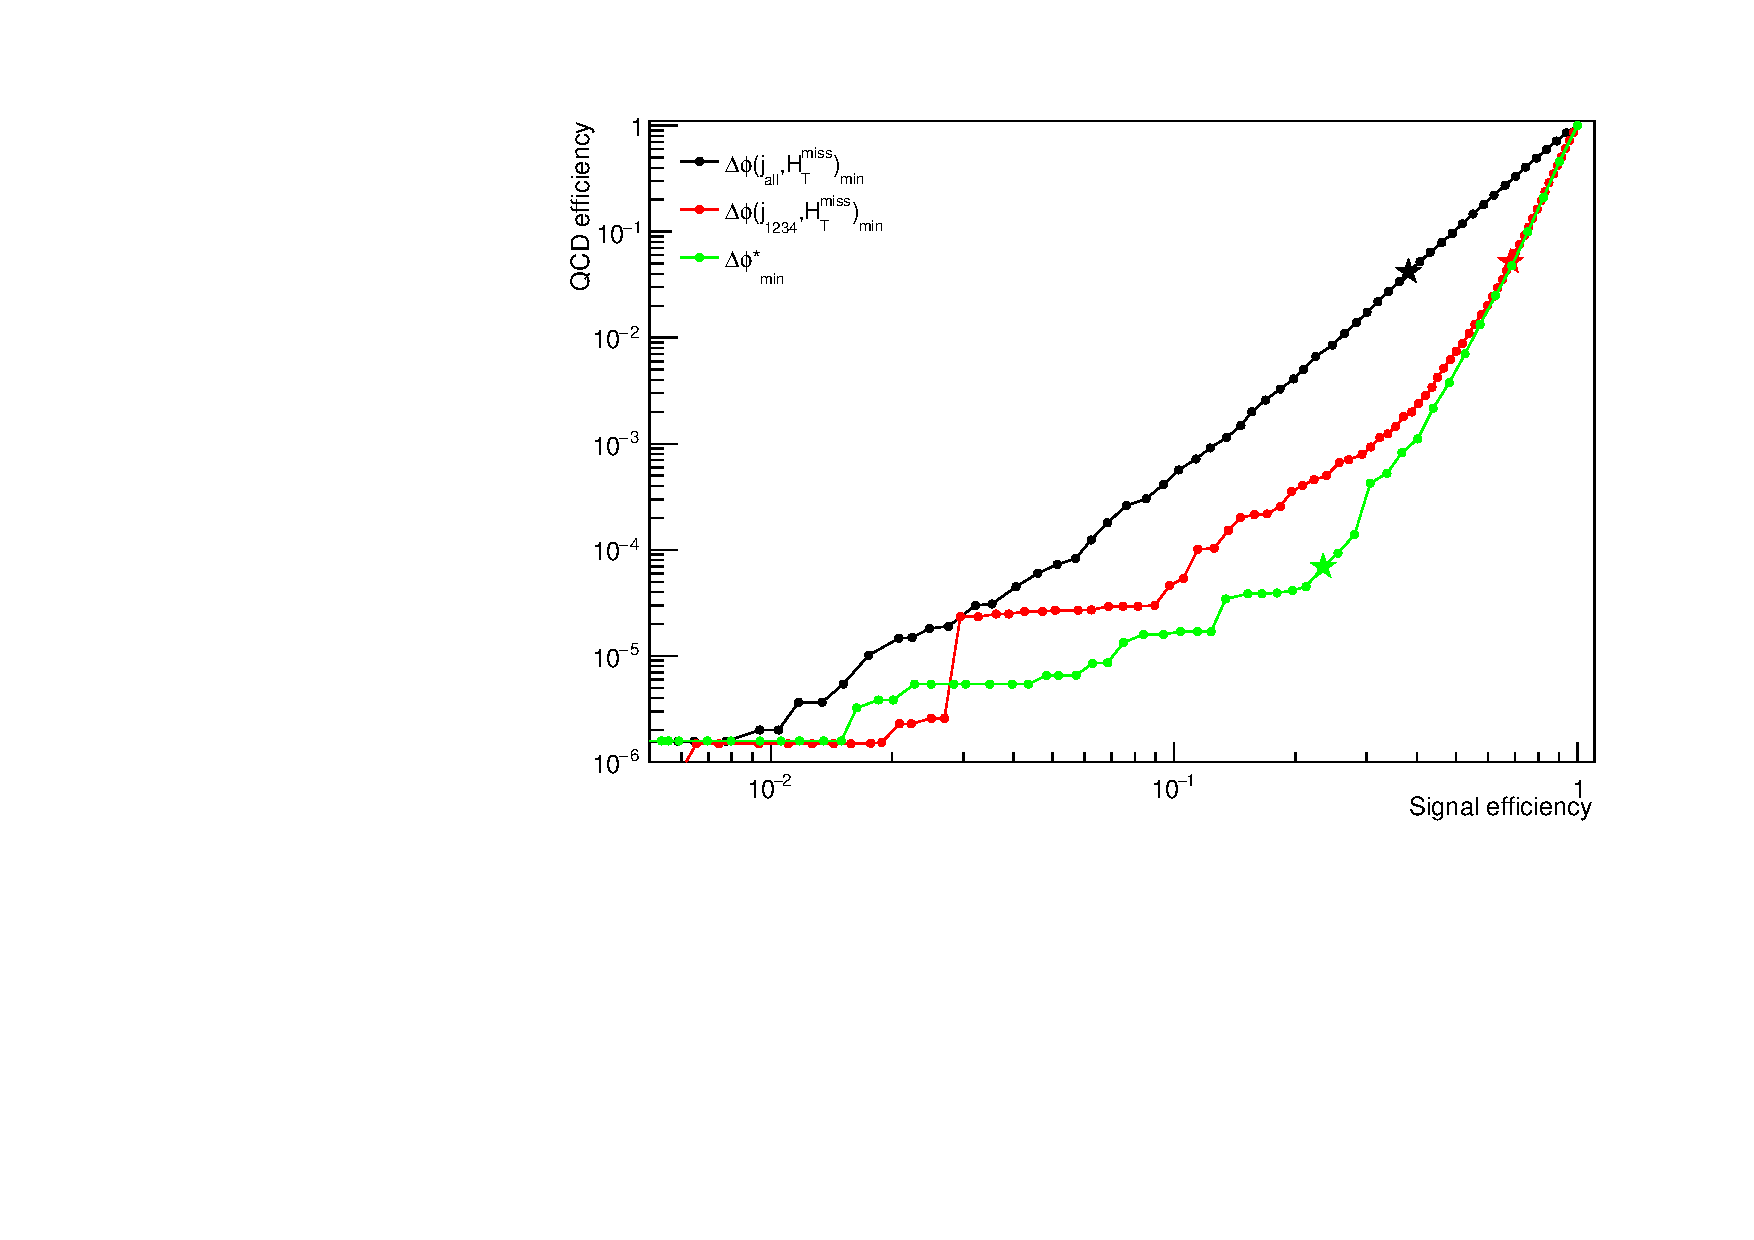
\includegraphics[width=0.5\textwidth]{figs/analysis/eventSelection/rateEffSignalQCD}
 } \\
 \caption{\bdphi, \dphimhtj and \dphimhtjall efficiency for simulation of processes with genuine
 \met vs QCD multijet background efficiency. The stars correspond to
 efficiencies with a cut of $0.5$ on each variable. A generic case of
 non-multijet process efficiency is considered in (a). In (b) we
 consider an uncompressed T1tttt model. This is the case in which \bdphi is
 expected to have the lowest efficiency due to the very high jet
 multiplicity of the model.}
 \label{fig:bDPhi_roc}
\end{figure}

Additionally the \bdphi variable displays robustness in the presence
of severe event mismeasurement. A mismeasurement is simulated by
artificially lowering the \pt of the jet that minimises the azimuthal
separation variable to 41~\gev. Due
to the removal of the probe jet from the computation of \bdphi, the
distribution of angular separation Fig.~\ref{fig:shifted_bDPhi_dist}
is remains unchanged under severe mismeasurement. The \dphimhtj
variable is sensitive to such mismeasurement as both \mht and the rank
of the leading four jets are affected, resulting in a broader
distribution with increased leakage
Fig.~\ref{fig:shifted_DPhiMht_dist}.

\begin{figure}[!h]
 \centering
 \subfloat[QCD \bdphi distribution with mismeasurement.\label{fig:shifted_bDPhi_dist}]{
 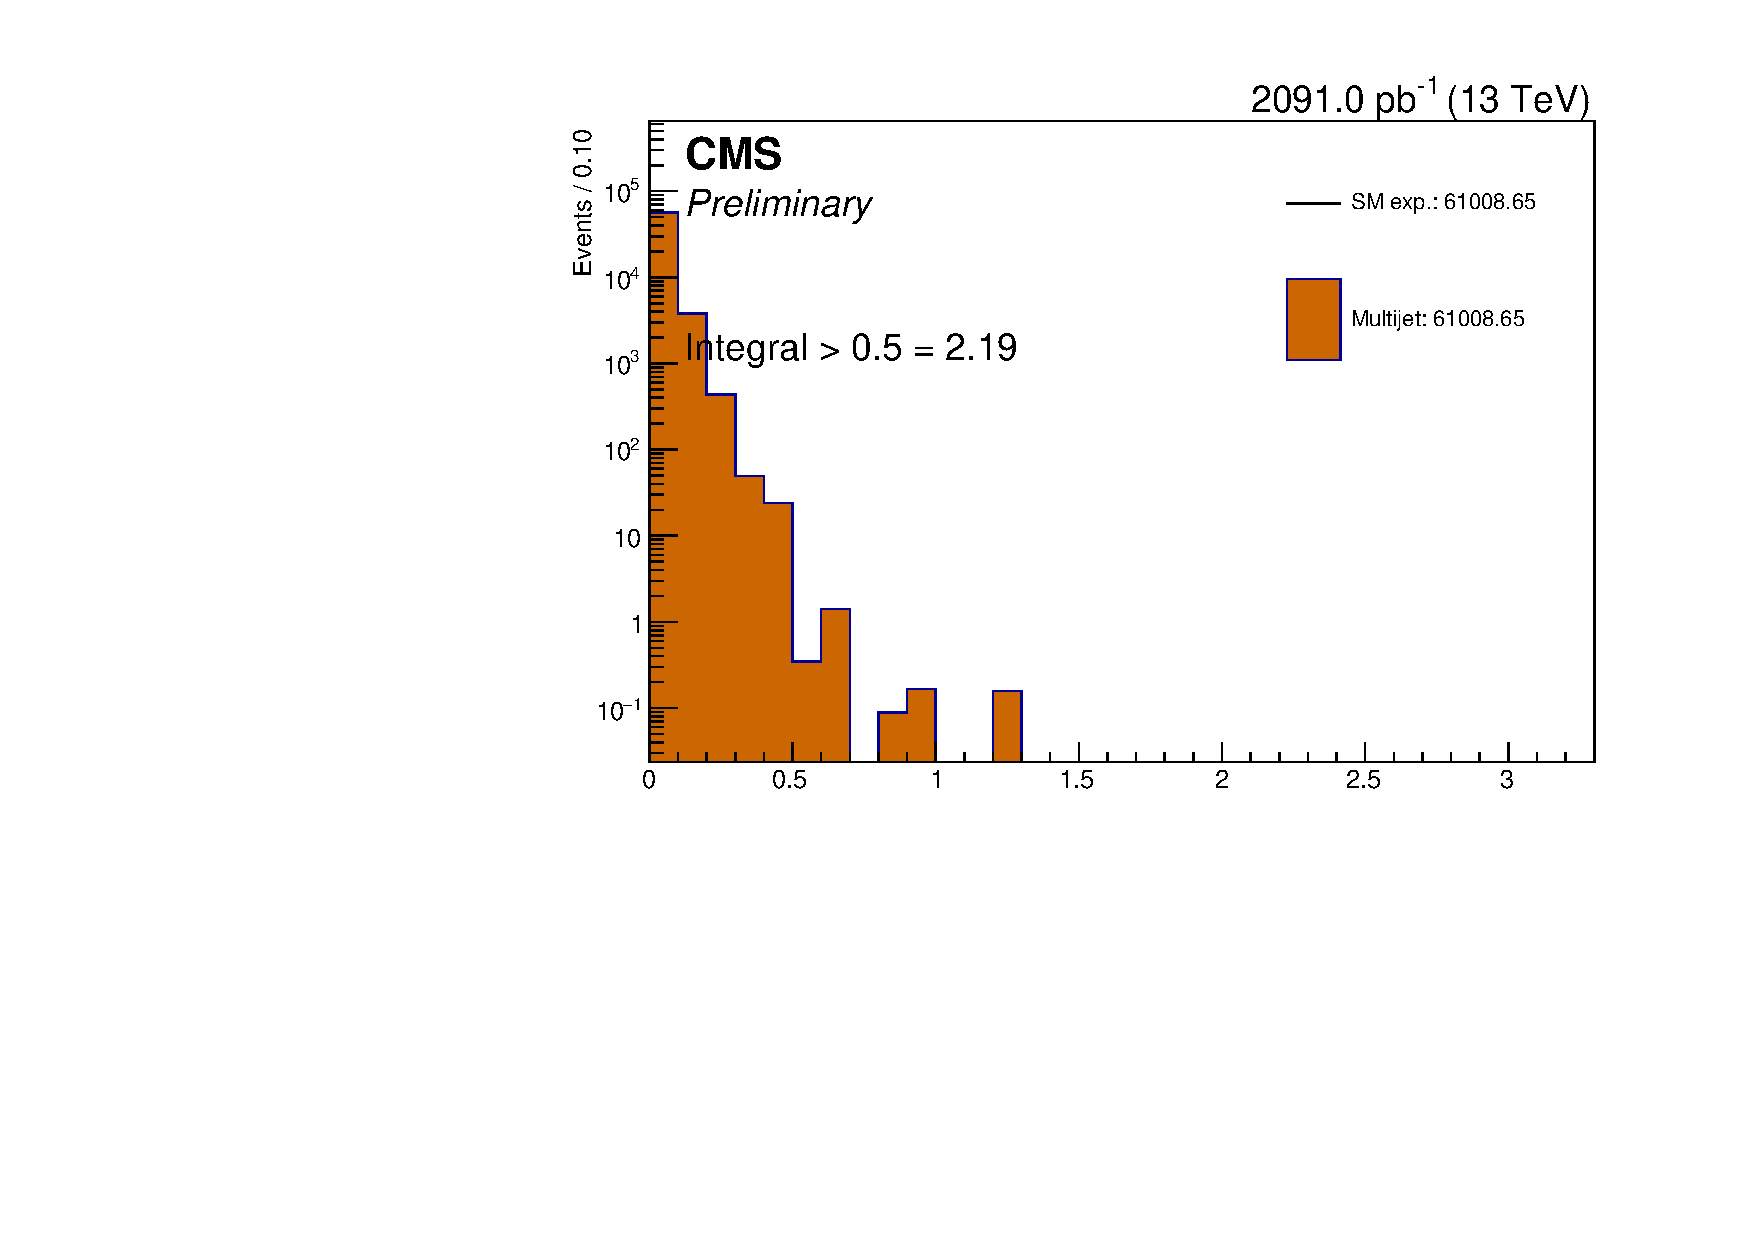
\includegraphics[width=0.5\textwidth]{figs/analysis/eventSelection/shiftedMinBDPhi_all_800}
 }
 \subfloat[QCD \dphimhtj distribution with mismeasurement.\label{fig:shifted_DPhiMht_dist}]{
 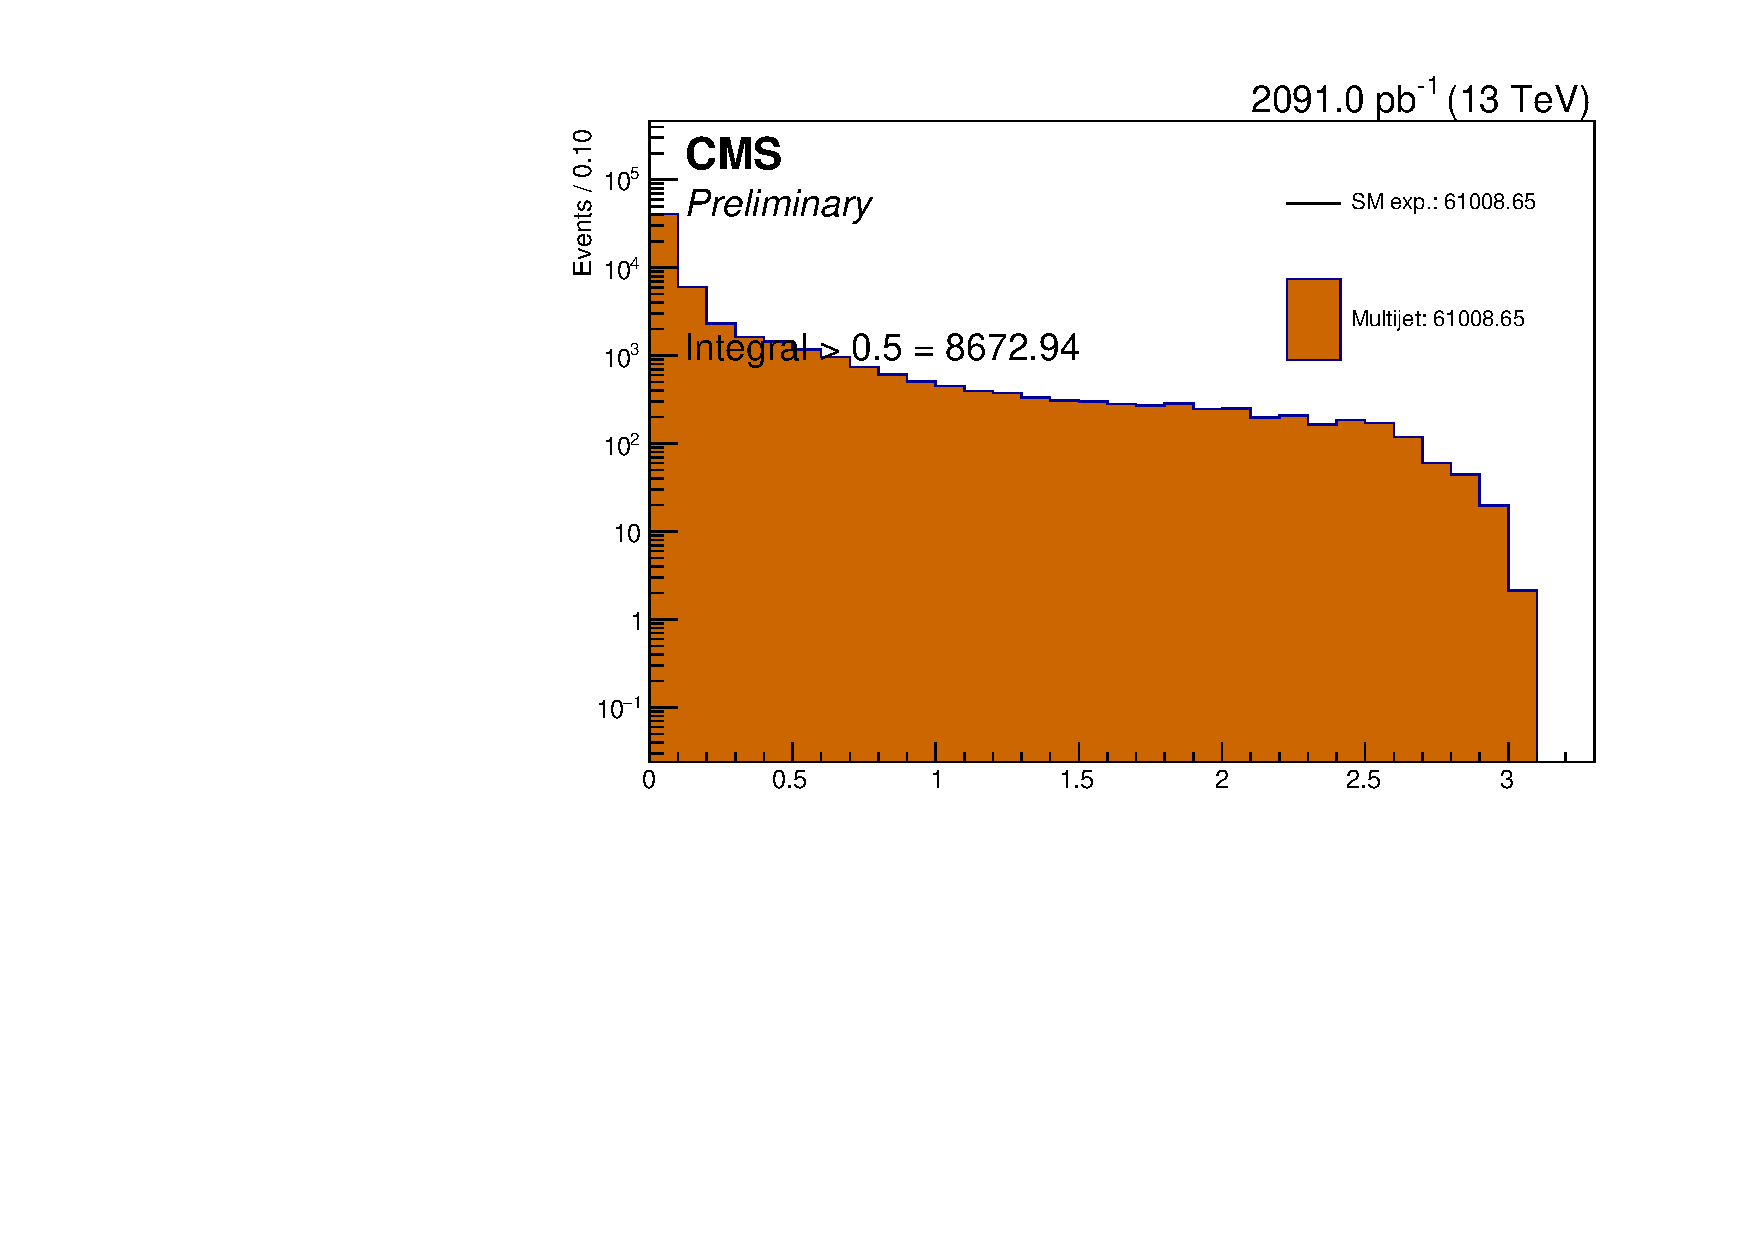
\includegraphics[width=0.5\textwidth]{figs/analysis/eventSelection/shiftedMinDeltaPhiMht_all_800}
 } \\
 \caption{\bdphi and \dphimhtj distributions of QCD multijet simulation
 after analysis selections for \scalht $> 800$ \GeV in the case of
 severe mismeasurement. The
 total number of events that pass a $\Delta\phi > 0.5$ selection of the
 respective quantity are indicated. (N.B. these plots were made with
 an older iteration of the analysis and have not been fully updated,
 although their conclusions remain true)}
 \label{fig:bDPhi_mismeasured}
\end{figure}

\subsection{The missing energy ratio \mhtmet}
\label{sec:mhtmet}

After requirements are made on the \alphat and \bdphi variables, the
majority of events with \MHT introduced from jet mismeasurement are
removed. However, this does not take account of events in which jets
fall below their reconstruction threshold, detailed for this analysis
in Sec.~\ref{sec:physobj}. If several jets fall just below threshold
they can fake a significant \MHT. There is a much lower threshold
on the particles that go into the \MET calculation than the jets that
go into the \MHT threshold. Therefore, a requirement on the ratio of
these two variables helps to remove the background from mismeasurement
that falls below threshold. The extent to which this removes the
remaining \QCD multijet backgroudn after the \alphat and \bdphi cuts
is shown in Fig.~\ref{fig:mhtDivMet}.
% removes soft stuff! given jet threshold

\begin{figure}
	\begin{center}
		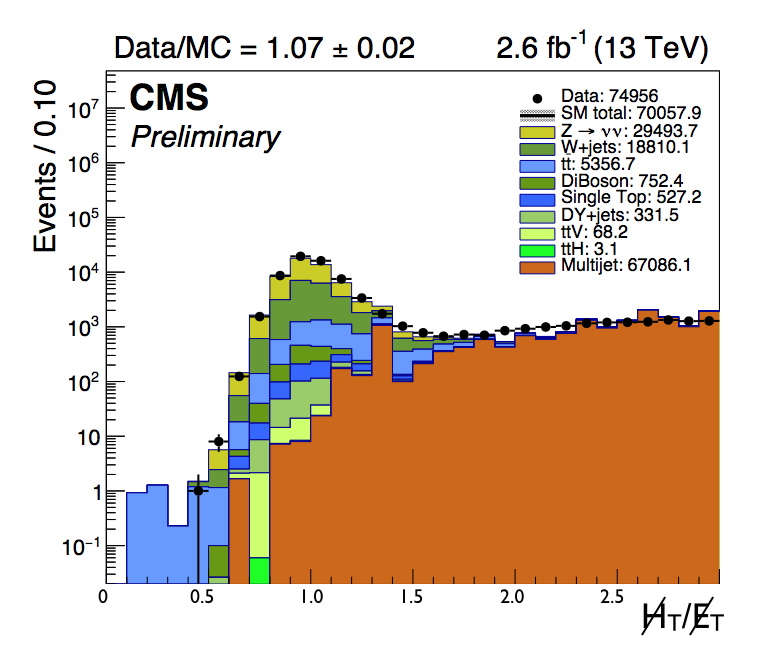
\includegraphics[width=0.5\linewidth]{figs/analysis/eventSelection/mht40_pt_Div_metNoX_pt_all_all_80X_noOverflow_scaled0p6}%alphaT1_bkgd}
	\end{center}
  \caption{The $\MHT/\MET$ distribution for \MC simulation with
  2.3~\ifb data overlaid, made at $\sqrt{s}=13~\tev$. The
  normalisation of the \MC simulation is scaled so the data and \MC
  match.}
	\label{fig:mhtDivMet}
\end{figure}

%%%%%%%%%%%%%%%%%%%%
\section{Physics objects} %day3
\label{sec:physobj}

The analysis makes use of physics objects that are reconstructed with
the algorithms described in Chapter~\ref{chap:reconstruction}. As
there are many different input parameters within each of the
algorithms, the specific details relevant to the analysis are
described in this section. Jets are reconstructed to characterise the
hadronic activity within the event, Muons, electrons and photons are
reconstructed for a signal region veto and for selecting the \emph{control
regions} that are used for background estimation, detailed in
Sec.~\ref{sec:controlregions}. \emph{Isolated tracks} are additionally
reconstructed to provide an extra type of lepton veto when the leptons
are not fully reconstructed.

\subsection{Jets}
\label{sec:evSel_jets}

Jets are defined as sets of particle-flow (PF) candidates clustered by
the anti-$k_{T}$ jet clustering algorithm with
a distance parameter of 0.4 (PFJets). \acf{CHS} is applied, charged
hadrons that can be traced back to \PU vertices are not clustered. The
four-vectors of the jets are then corrected with the procedure
outlined in Sec.~\ref{sec:reco_jec}.

The \emph{loose} working point jet quality criteria is chosen.  The cuts
are listed in Tab.~\ref{tab:loose-jet-id}. All jets are required to
contain at least part of their energy within the \ECAL and \HCAL and
must consist of at least one of different types of particles. This is
effective at removing fake jets that are the result of detector noise.
In addition, a dedicated selection is applied to reject \emph{beam
halo} candidate events, which manifest themselves as a single energy
deposit in the calorimeters. A requirement that at least 10\% of the
energy of the jet comes from charged hadrons is enough to negate this
effect.
%maybe show plots here?

\begin{table}[ht!]
  \caption{The \emph{loose} jet ID requirements. \label{tab:loose-jet-id}}
  \centering
  \begin{tabular}{ ccc }
    \hline
    \hline
    Variable & cut & notes \\ \hline
    \multicolumn{3}{c}{$-3.0 < \eta_{\mathrm{jet}} < 3.0$} \\ \hline    
    Neutral Hadron Fraction & $<0.99$ & - \\
    Neutral Electromagnetic Fraction & $<0.99$ & - \\
    Number of constituents & $>1$ & - \\
    Charged Hadron Fraction & $>0$ & only for $|\eta_{\mathrm{jet}}| < 2.4$ \\
    Charged Multiplicity & $>0$ & only for $|\eta_{\mathrm{jet}}| < 2.4$ \\
    Charged Electromagnetic Fraction & $<0.99$ & only for $|\eta_{\mathrm{jet}}| < 2.4$ \\ \hline
    \multicolumn{3}{c}{$|\eta_{\mathrm{jet}}| > 3.0$} \\ \hline        
    Neutral Electromagnetic Fraction & $<0.90$ & - \\
    Number of Neutral Particles & $>10$ & - \\
    \hline
    \hline
  \end{tabular}
\end{table}

Jets are also $b$-tagged with the \emph{medium} working point of the
algorithm described in Sec.~\ref{sec:reco_btag}. This is obtained with
a cut of $>$ 0.800 on the algorithm discriminator variable. This
results in a gluon/light-quark mis-tag rate of $\sim$1 \% (where
\emph{light} means $u$, $d$ and $s$ quarks), a charm-quark mis-tag
rate of $\sim$10 \% and a b-quark b-tag efficiency of about 60 \%. 


\subsection{Muons}
\label{sec:muon-id}
Two types of selection are made on muons depending on whether they are
used to carry out the veto in the signal region or used for selecting
one of the control regions. A tighter criteria is used for the control
region and muons are required to be well isolated. The muon is
required to have been
reconstructed with the \emph{global} algorithm, as detailed in
Sec.~\ref{sec:muons_reco}. The muon is required to consist of a track
with at least 5 inner layer hits, a good fit, good compatibility with
the primary vertex and significant muon chamber hits. The isolation in
the control region uses the \emph{relative isolation} algorithm
defined in Sec.~\ref{sec:reco_iso} with \emph{effective-area}
correction, it is required that $I^{\textrm{rel}}<0.15$.  

For the purpose of vetoing muons in the signal region, a looser
working point is used, which provides $\sim$ 98 $\%$ efficiency. The
muon is just required to be classified within the \PF algorithm and
reconstructed with the \emph{global} or \emph{tracker} muon
algorithms. The
\emph{mini-isolation} algorithm is utilised with effective-area \PU
correction $I^{\textrm{rel}}_{\textrm{mini}} < 0.2$. The reconstructed
muon must have a $\pT>10~\gev$ and be within $|\eta|<2.1$.

\subsection{Photons}
\label{sec:photon-id}

Photons are identified according to a \emph{tight} working point
definition ($\sim$ 71 $\%$ efficiency) and required to be well
isolated.  A \PF-based isolation which considers neutral and charged
hadrons separately is used with a cone size $\Delta R$
$<$ 0.3 and $\rho\times A_{eff}$ corrections are applied to remove the
effects of pileup.  Table \ref{tab:photon-id-gamma}
summarises the isolation selection used. There are additional
requirements on the ratio of \HCAL and \ECAL deposits and the
kinematics of the deposits within the \ECAL. The reconstructed
photon must have a $\pT>25~\gev$ and be within $|\eta|<2.5$.

\begin{table}[ht!]
  \caption{Photon isolation criteria (\emph{tight} working point). The
  energy of particles within the isolation cone must be less than the
  value in the column.\label{tab:photon-id-gamma}}
  \centering
  \footnotesize
  \begin{tabular}{ ccc }
    \hline
    \hline
    Categories                    & Barrel                             & EndCap                             \\
    \hline
    PF charged hadron isolation   & 1.66 GeV & 1.04 GeV                          \\
    PF neutral hadron isolation   & 0.14 + $ e^{0.0028 \times \pt^{\gamma} + 0.5408}$  &  3.89 + 0.0172 $\times$ $\pt^{\gamma}$\\
    PF photon isolation           & 1.40 + 0.0014 $\times$ $\pt^{\gamma}$ & 1.40 + 0.0091 $\times$ $\pt^{\gamma}$ \\
    \hline
    \hline
  \end{tabular}
  \end{table}

\subsection{Electrons}
\label{sec:electron-id}

In order to veto electrons a \emph{loose} working point definition
($\sim$ 90 $\%$ efficiency) is used. There are requirements on the
ratio of \HCAL and \ECAL deposits, criteria to remove photons that
have converted within the tracker, a minimum number of tracks required
and kinematic requirements on the deposit within the \ECAL. Electrons
are also require required to be isolated with the effective-area
corrected mini-isolation algorithm.  Isolated electrons are defined by
$I^{\textrm{rel}}_{\textrm{mini}} < 0.1$. The reconstructed electron
must have a $\pT>10~\gev$ and be within $|\eta|<2.5$.

% Table \ref{tab:ele-id} summarises the identification 
% selection used. 
%
% \begin{table}[h!]
%   \caption{Electron identification (``tight'' working point).\label{tab:ele-id}}
%   \centering
%   \footnotesize
%   \begin{tabular}{ lcc }
%     \hline
%     \hline
%     Categories                                               & Barrel    & EndCap    \\
%     \hline
%     $\Delta \eta_{In}$                                       & 0.0105   & 0.00814  \\
%     $\Delta \phi_{In}$                                       & 0.115    & 0.182  \\
%     $\sigma_{i\eta i\eta}$                                   & 0.0103    & 0.0301  \\
%     H/E                                                      & 0.104    & 0.0897   \\
%     d0 (vtx)                                                 & 0.0261    & 0.118  \\
%     dZ (vtx)                                                 & 0.041    & 0.822  \\
%     $\lvert(1/E_{\textrm{ECAL}} - 1/p_{\textrm{trk}})\rvert$ & 0.102     & 0.126  \\
%     Missing hits (inner tracker)                             & 2         & 1         \\
%     Conversion veto                                          & yes       & yes   \\
%     \hline
%     \hline
%   \end{tabular}
%   \end{table}


\subsection{Isolated tracks}
\label{sec:SIT}

A \ac{SIT} can be used to identify W bosons through
their leptonic decays: W $\rightarrow$ $\mu \nu$, W $\rightarrow$
$e\nu$, and W $\rightarrow$ $\tau$($\rightarrow l$) $\nu$.  Single
prong decays of the tau lepton can also be identified: W $\rightarrow$
$\tau$ ($\rightarrow$ h$^{\pm}$ + n$\pi^{0}$) $\nu$.  A single
isolated track comprises a charged PF candidate with $\Pt > 10 \gev$,
$\Delta z(\mathrm{track}, \mathrm{\ac{PV}}) < 0.05 \, \mathrm{cm}$ and with
a relative isolation smaller than 0.1, where the isolation is
determined from the sum of the \Pt of the charged PF candidates within
$\Delta R < 0.3$.
%Events in the signal region and all control regions (ignoring the
%selected muons) containing a SIT candidate identified with these
%criteria are vetoed.


\subsection{Energy sums}

Missing transverse momentum (\MET) is reconstructed as described in
Sec.~\ref{sec:met_reco} and the the Type-I \MET energy correction is applied.
The \met is used in the definition of 
the transverse mass, $M_{T}$, which is in turn used as part of
the selection criteria that define the single muon control sample 
(Sec.~\ref{sec:controlregions}), and for the $\mhtmet$ cleaning
filter, described in Sec.~\ref{sec:mhtmet}.

The \HT and \MHT energy sums are constructed with the jets outlined in
Sec.~\ref{sec:evSel_jets}, which are subject to the kinematic requirements of
$\pT>40$~\gev and $|\eta|<3$.

%%%%%%%%%%%%%%%%%%%%
\section{Trigger strategy}

As \SUSY models have a lot of freedom in how they are manifest, a
guiding principle of the analysis is to maintain acceptance of as much
phase space as possible. Despite some \SUSY models being ruled out at
energies $O(100)$~\gev, models with compressed spectra are still poorly
constrained in this regime. The trigger strategy therefore revolves
around maintaining as low an energy threshold as possible given the
very high rate of \QCD multijet processes. To select for events with
significant hadronic activity and missing energy, triggers are used
that rely on the \HT and \MHT of the events. Additionally, including
topological variables, such as \alphat, in the \HLT allow events to be
collected with $\HT$ as low as $200~\gev$.

\bf{FIXME} The L1 paths we use and why - ask christian
%L1

To collect events that are of general use to hadronic analyses the
$\HT$ of each event is reconstructed within the \HLT. This is carried
out with a custom form of \PF, that is designed to work in a way that
is quick enough given the time the trigger has to make a decision. To
further help with this timing constraint, the \HT is calculated with
jets clustered from only calorimeter deposits and a looser constraint
is made, reducing the load on the \PF reconstruction. This allows for
all events that pass $\HT>800~\gev$, calculated by the \HLT,
to be collected. When carrying out full online reconstruction, this
results in a $\sim 100\%$ efficiency for events with an offline
$\HT>900~\gev$. 

To be able to efficiently collect events with lower
values of \HT, the \alphat variable is calculated within the \HLT. A
requirement is made on both \alphat and \HT for a series of different
\HT thresholds. These requirements are chosen to limit the rate of the
\alphat-\HT triggers to an acceptable level, while maintaining low
acceptance of events with low \HT. 

There are also general purpose missing energy triggers that require
both an \MHT and \MET threshold to be surpassed within the \HLT.
Including events selected by these triggers helps to increase the
efficiency across the board. These variables, however, are quite sensitive to
running conditions and mismeasurement, so are not as robust against
the \HLT rate as the \alphat-\HT triggers. The full list of
triggers used to collect data for the signal region of the \alphat
analysis can be seen in Tab.~\ref{tab:triggers}.

\bf{FIXME} The HLT paths we use (in a table) - including the CR
triggers

The events in the control regions are collected with muon or photon
triggers, where the \HLT requires at least one of these objects above
a certain energy threshold threshold. Due to the lower rate of events
containing leptons, these triggers are at full efficiency for their
requirements in the analysis. The specific triggers used are listed in
Tab.~\ref{tab:triggers}.

%%%%%%%%%%%%%%%%%%%%
\section{Pre-selection}%day4
\label{sec:preselection}

To ensure that all events considered by the analysis have a
significant hadronic activity and missing energy a pre-selection is
carried out on all events considered in the signal and control
regions. Events are required to contain at least one $p_T>100$~GeV,
with all other jets being considered if they have $p_T>40$~GeV and are
well reconstructed in the central region, $|\eta|<2.4$. If any jets
fall outside the $\eta$ range, the event is vetoed. This ensures there
is no significant energy deposited within the region of the detector
with no tracker, which will not be reconstructed as well and is more
prone to mismeasurement. As signatures of \BSM physics typically occur
through particles at a high mass scale, they are expected to deposit
most of their energy centrally. For this reason this \emph{forward jet
veto} does not significantly effect the signal efficiency for most
models. The \QCD multijet background consists of many
soft scattering events, which typically deposit a significant
proportion of energy within the forward region. As this is the case
the forward jet veto helps to improve the ratio of signal to
background.

Significant hadronic activity is selected by requiring $H_T>200$~GeV.
This cut is primarily motivated by the trigger threshold, it is the
lowest \HT value that can be reached with a reasonable trigger rate
and efficiency. To ensure there is significant missing energy, the
main \BSM signature of interest, it is required that $\MHT>130~\gev$.
This threshold is chosen as roughly equivalent to the magnitude of the
\MET requirement made by the \alphat cuts within the signal region
when there is no significant mismeasurement. 
%could expand on this with formula?

Additionally, to remove events with significant hadronic energy
deposits that have not been reconstructed as jets a requirement is
made on the \MHT and \MET ratio $\mhtmet<1.25$, motivated in
Sec.~\ref{sec:mhtmet}. When this requirement is made for the control
regions, the \MET is reconstructed without a contribution from the
leptons or photons that define the region. This ensures a fair
comparison with \MHT and allows the lepton to simulate the missing
momentum in the events in the signal region.

To further ensure the beam conditions or reconstruction effects have
not, centrally defined filters are applied by analyses that rely
on \MET, including the analysis defined in this chapter. The filters
used are designed to remove the instances of fake \MET while retaining
a high efficiency for real physics events, they are described in the
following.
\begin{itemize}
\item{The primary vertex must be well reconstructed within
$|z|<=24$~cm of the proton collision region and $d_{xy}<2$~cm from the
beam line}
\item{Beam interactions exterior to the detector, beam halo effects,
are removed by vetoing events with \ac{CSC} and calorimeter energy
deposits consistent with interactions from particles outside the
detector.}
\item{Noise, caused by particle interactions with the read-out system,
and dead regions within the \HCAL are removed with the \emph{HBHE
noise and isolation filters}}
\item{Anomalous signals within the \ECAL endcap supercrystals are removed
with the \emph{\ECAL Endcap SC Noise filter}}
\item{Events with misidentified straight tracks that are reconstructed
to have a large \pT are removed by the \emph{bad track filter}.}
\item{}
\end{itemize}

A summary of the pre-selection requirements is in
Tab.~\ref{preselection}.

\begin{table}[h!]
  \topcaption{Summary of the pre-selection criteria.}
  \label{tab:pre-selections}
  \centering
  \footnotesize
  \begin{tabular}{ ll }
    \hline
    \hline
    Selection                     & Requirement                     \\
    \hline
    ``MET filters''               & \parbox[t]{10cm}{Primary Vertex, CSC Beam Halo,
      HBHE Noise and Isolation, \\ ECAL Endcap SC Noise, ECAL TP, bad
      track filter}         \\
    Jet acceptance                & $\PT > 40\gev$, $|\eta| < 2.4$                      \\
    Lead jet acceptance           & $\PT > 100\gev$, $|\eta| < 2.4$                   \\
    Forward jet veto              & $\PT > 40\gev$, $|\eta| > 2.4$                     \\
    \HT requirement               & $\HT > 200\gev$                  \\
    \mht requirement              & $>130\gev$         \\  
    \mhtmet requirement              & $<1.25$         \\  
    \hline
    \hline
  \end{tabular}
\end{table}

\section{The signal region}
\label{sec:signalregion}

%variable alphaT
%bDphi

\section{The control regions}
\label{sec:controlregions}

%describe and motivate each of them as in AN

\section{Event categorisation}
Events are categorised based on the number of
jets, the number of jets with a reconstructed b-quark and the value of
$H_T$.
%the jet topology, symmetric, asymmetric etc.

%%%%%%%%%%%%%%%%%%%%
\section{Corrections to simulation} %day5

% mention tails of Njet and ETmiss are hard to simulate?


\subsection{Trigger efficiencies}

%as we maintain low thresholds operate near the trigger turn on: corrections
% put in trigger efficiency plots

\subsection{Scale factors}

% SFs from muons etc...

%%%%%%%%%%%%%%%%%%%%
%\section{Further optimisation of event selection}
% something about minChi here?
